% !TeX program = lualatex
% !TeX root = luaking.tex
% !TeX encoding = UTF-8
% !TeX spellcheck = cs_CZ
%---------------------------------------------------------------------------------------------------
% file fey1ch21.tex
%---------------------------------------------------------------------------------------------------
%=========================== Kapitola: Harmonický oscilátor ========================================
\setchaptertoc
\chapter{Harmonický oscilátor}\label{fyz:IchapXXI}
  \section{Lineární diferenciální rovnice}\label{fyz:IchapXXIsecI}
    Kurz studia fyziky se obvykle dělí na tématické části jako například mechanika, elektřina,
    optika atd., přičemž se studují jedna za druhou. Například v našem kurzu jsme se zatím většinou
    zabývali mechanikou. Znovu a znovu se však stává podivná věc: rovnice, jež se objevují v různých
    odvětvích fyziky, a dokonce i v jiných vědách, jsou často téměř stejné. Mnohé jevy mají proto
    své analogie v těchto různých odvětvích. Jako jednoduchý příklad uveďme, že šíření zvukových vln
    je v mnohém podobné šíření světelných vln. Při podrobném studiu akustiky zjistíme, že studujeme
    téměř totéž, jako kdybychom se podrobně zabývali studiem optiky. Studium nějakého jevu v jedné
    oblasti tak může rozšířit naše vědomosti v jiné oblasti. Nejlépe bude, když si od začátku
    uvědomíme, že takováto rozšíření jsou možná, neboť' jinak by možná někdo neviděl důvod, proč
    ztrácet čas a energii s něčím, co se zdá být jen malou částí mechaniky.
    
    Harmonický oscilátor, který se chystáme studovat, má blízké analogie v mnoha jiných odvětvích.
    Ať už začneme s příkladem závaží na pružině, kyvadla s malou výchylkou nebo jiných mechanických
    zařízení, studujeme ve skutečnosti určitou \textbf{diferenciální rovnici}. Tato rovnice se ve
    fyzice i v jiných vědách objevuje vždy znovu a znovu. Ve skutečnosti je částí tolika jevů, že
    její studium si zaslouží naši pozornost. Některé jevy, které popisuje tato rovnice, jsou
    oscilace tělesa na pružině, oscilace náboje v elektrickém obvodu, oscilace ladičky vytvářející
    zvukové vlny, vibrace elektronů v atomu vytvářející světelné vlny, rovnice činnosti takového
    servosystému, jakým je termostat regulující teplotu, komplikované interakce v chemických
    reakcích, růst kolonie bakterií interagujících s dodávanou potravou a otravnými látkami, které
    bakterie produkují, lišky, požírající králíky žeroucí trávu atd. Všechny tyto jevy probíhají
    podle rovnic, jež jsou si velmi podobné, a to je důvod, proč se tak podrobně zabýváme
    mechanickým oscilátorem. Tyto rovnice jsou \textbf{lineárními diferenciálními rovnicemi s
    konstantními koeficienty}. Lineární diferenciální rovnice s konstantními koeficienty je rovnice,
    která se skládá ze součtu více členů, přičemž každý člen je derivací závisle proměnné podle
    nezávisle proměnné vynásobený nějakou konstantou. Takže
    \begin{equation}\label{fyz:eq727}
      andnx/dtn+an−1dn−1x/dtn−1+⋯+a1dx/dt+a0x=f(t)
    \end{equation}
  
  \section{Harmonický oscilátor}\label{fyz:IchapXXIsecII}
  \section{Harmonický pohyb a pohyb po kružnici}\label{fyz:IchapXXIsecIII}
  \section{Počáteční podmínky}\label{fyz:IchapXXIsecIV}
  \section{Nucené kmity}\label{fyz:IchapXXIsecV}
  \section{Příklady a cvičení}\label{fyz:IchapXXIsecVI}

    \begin{figure}[ht!] %\ref{fyz:fig246}
      \centering
      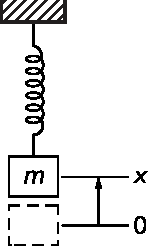
\includegraphics[width=0.3\linewidth]{fyz_fig246.pdf}
      \caption{Těleso upevněné na pružině - jednoduchý příklad harmonického oscilátoru
               (\cite[s.~287]{Feynman01})}
      \label{fyz:fig246}
    \end{figure}

    \begin{figure}[ht!] %\ref{fyz:fig247}
      \centering
      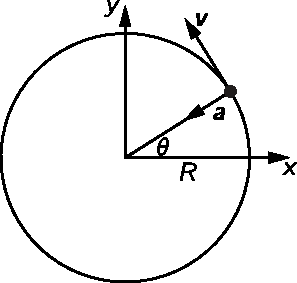
\includegraphics[width=0.5\linewidth]{fyz_fig247.pdf}
      \caption{Částice pohybující se po kruhové dráze konstantní rychlostí
               (\cite[s.~290]{Feynman01})}
      \label{fyz:fig247}
    \end{figure}

    \begin{figure}[ht!] %\ref{fyz:fig248}
      \centering
      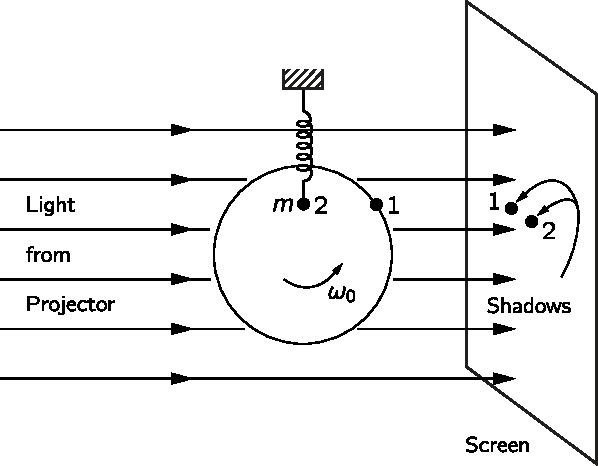
\includegraphics[width=0.5\linewidth]{fyz_fig248.pdf}
      \caption{Demonstrace ekvivalence jednoduchého harmonického pohybu a rovnoměrného pohybu po 
               krunici
               (\cite[s.~290]{Feynman01})}
      \label{fyz:fig248}
    \end{figure}

    \todo[inline]{Kapitola fey1ch21 je zcela prázdná, pouze obrázky}   
%} %tikzset
%---------------------------------------------------------------------------------------------------